\documentclass{article}

\usepackage{iclr2026_conference}
\usepackage{times}

\usepackage{graphicx}
\usepackage{booktabs}
\usepackage{amsmath,amssymb}
\usepackage{microtype}
\usepackage{enumitem}
\usepackage{placeins}
\usepackage{xurl}
\usepackage{needspace}

\hbadness=10000
\hfuzz=20pt

\setlength{\textfloatsep}{8pt plus 2pt minus 2pt}
\setlength{\floatsep}{8pt plus 2pt minus 2pt}
\setlength{\intextsep}{8pt plus 2pt minus 2pt}
\setlength{\abovecaptionskip}{4pt}
\setlength{\belowcaptionskip}{0pt}

\input{math_commands.tex}

\title{Prompt-Level Drift as an Operational Monitoring Problem:\\
Schema Failure Cliffs and Judge-Version Risk in Artifact-Grounded Evaluation}

\author{Yuchen Zhu \\
Shanghai University \\
\texttt{zyc20070222@gmail.com}
}
\iclrfinalcopy
\newcommand{\Astruct}{A\_structure}
\newcommand{\Bsnap}{B\_snapshot\_constraint}
\newcommand{\Cact}{C\_actionability}
\newcommand{\Dcomp}{D\_completeness}
\newcommand{\Edrift}{E\_drift\_failure}

\begin{document}
\flushbottom
\maketitle

\begin{abstract}
Prompt templates are routinely edited in deployed LLM systems and evaluation pipelines, often treated as ``non-functional'' refactors.
We reframe \emph{prompt-level drift} as an \emph{operational monitoring} problem: minimal prompt perturbations can trigger discontinuous schema violations, degrade instruction following, and even shift conclusions when the \emph{judge prompt}---the measurement instrument---changes.
Methodologically, we study these failures through an artifact-grounded evaluation pipeline built on a fixed evidence snapshot, where preserved outputs, versioned judge/model slices, processed records, and summary tables form a one-way audit chain.
Across six preserved judge/model slices under a baseline judge (three judge models scoring outputs from the other two providers), reducing contract salience from explicit to implicit increases schema hard-breaks (\Astruct$=0$) from $8/48$ (16.7\%) to $34/48$ (70.8\%) and drops the mean total score from 7.69 to 2.75 (max total = 10).
We further show judge-version sensitivity on \emph{identical preserved outputs}: for one overlapping slice (ChatGPT-as-judge scoring Gemini outputs under implicit triggers), the hard-break rate shifts from $8/8$ (v0) to $0/8$ (v1/v2), and the mean total score shifts from 0.0 (v0) to 8.0 (v1) to 10.0 (v2).
These patterns motivate CAO-style change control: pin prompt and judge versions, monitor interface validity, and prohibit pooling metrics across judge versions.
\end{abstract}

\section{Introduction}
LLM applications commonly rely on prompts not only to specify the task, but also to enforce output \emph{interfaces} required by downstream tooling (e.g., fixed sections, JSON-like blocks, or other schemas).
In practice, prompts are edited frequently: teams reorder constraints, ``clean up'' formatting, or paraphrase evaluation rubrics.
A tacit assumption is that these edits are safe---that behavior and measured quality change smoothly.

This paper challenges that assumption from an engineering perspective.
We study \emph{prompt-level drift} as an operational risk surface with three incident types:
(i) \textbf{interface incidents} (schema failures that break parsers),
(ii) \textbf{quality incidents} (instruction-following degradation under minimal edits), and
(iii) \textbf{measurement incidents} (score shifts caused by judge prompt changes rather than generator changes).
Our goal is \emph{not} to propose a new evaluator or a more robust prompt.
Instead, we aim to make prompt drift \emph{monitorable and auditable} in a Catch--Adapt--Operate setting.

Methodologically, we ground this framing in an artifact-grounded evaluation pipeline (Figure~\ref{fig:pipeline_overview}): prompt variants produce preserved raw outputs, judges produce versioned judge/model slices, and reporting is derived through processed records and summary tables.
This one-way evidence chain makes prompt-drift incidents auditable without re-running generators or judges and turns qualitative prompt edits into monitorable operational events.

\begin{figure*}[t]
\centering
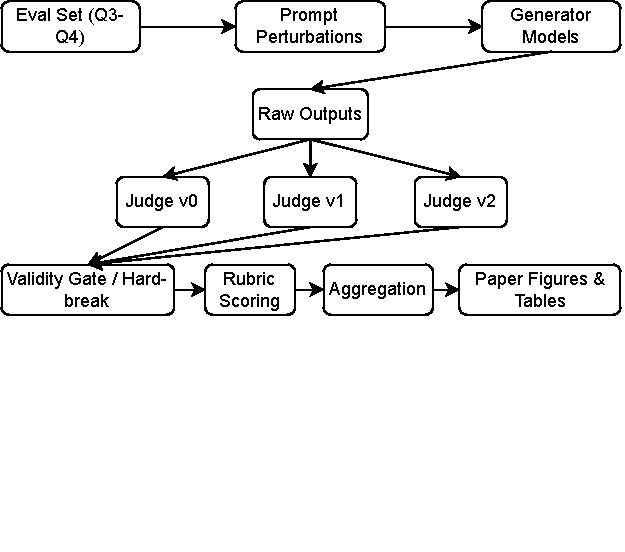
\includegraphics[width=\textwidth]{figures/fig_pipeline_overview.pdf}
\caption{\textbf{Evaluation pipeline overview.} A visual summary of the one-way evidence chain from prompt variants to raw outputs, versioned judge/model slices, processed records, and summary tables.}
\label{fig:pipeline_overview}
\end{figure*}

\paragraph{Contributions.}
\begin{itemize}[leftmargin=1.2em, itemsep=2pt, topsep=2pt]
  \item \textbf{Operational framing of prompt drift.} We treat prompt edits as configuration drift and define incident-level outcomes (schema hard-breaks, dimension-level degradation, judge-version sensitivity).
  \item \textbf{Artifact-grounded evaluation pipeline.} We introduce a one-way evidence chain from prompt variants to preserved outputs, versioned judge/model slices, processed records, and summary tables, enabling auditability without re-running generators or judges.
  \item \textbf{Operational risk patterns under minimal perturbations.} Using preserved outputs and versioned judges, we surface schema failure cliffs, broad rubric-dimension degradation, and judge-version sensitivity as concrete monitoring risks.
\end{itemize}


\section{Related Work}
We connect three practice-facing threads: LLM-as-judge reliability, prompt robustness/interface contracts, and drift monitoring.

\paragraph{LLM-as-judge reliability.} LLM evaluators can be biased and prompt-sensitive, motivating controls and debiasing \citep{zheng2023judging,chiang2024chatbotarena,dubois2024lengthcontrolled,chen2024humans,mukherjee2025metaevalcollapse,feuer2025judgmentnoise}. We treat judge prompting as \emph{instrumentation drift} and emphasize an evidence chain from prompts to outputs to reported summaries.
\paragraph{Prompt robustness and interface contracts.} Robustness work studies sensitivity to surface perturbations \citep{zhu2023promptrobust}; we focus on non-adversarial refactors that break downstream interfaces, operationalized via schema hard-breaks (\Astruct$=0$).
\paragraph{Monitoring under drift.} Monitoring emphasizes slice-aware diagnostics and change control \citep{kang2020modelassertions,yao2022wildtime,baby2025adapting,hao2025nazar}; CAO suggests prompts and judges be versioned dependencies with guardrails. We contribute concrete, auditable failure patterns under minimal edits.

\section{Problem Setup: Prompt Drift as Operational Risk}
\subsection{Prompt edits as configuration drift}
We define \textbf{prompt-level drift} as any change to generator or judge prompts that preserves the intended task but changes surface form-wording, ordering, markers, delimiters, or emphasis.
Operationally, such edits are common during maintenance (policy updates, refactors, localization, ``make it cleaner'') and can be shipped without model changes.
Prompt drift is therefore a first-class monitoring input: it can create incidents even when the model and data are stable.

\subsection{Output contract and schema hard-breaks}
Our evaluated generator prompts require a fixed \textbf{three-section output contract}.
The rubric includes a structure dimension \Astruct{} scored in $\{0,1,2\}$.
We define a \textbf{schema hard-break} as \Astruct$=0$, meaning the output does not satisfy the interface contract (e.g., missing required sections or invalid ordering).
Hard-breaks are operationally meaningful because they represent \emph{interface outages}: downstream systems cannot safely consume the output regardless of content quality.

\subsection{Incident taxonomy and monitoring targets}
We monitor prompt drift through three incident targets, each derived from the reported metrics:
\begin{itemize}[leftmargin=1.2em, itemsep=2pt, topsep=2pt]
  \item \textbf{Interface validity:} schema hard-break rate $\mathrm{HBR}(\pi)$ (Eq.~\ref{eq:hbr}) and section-level validity gates.
  \item \textbf{Quality degradation:} dimension means $\mu_d(\pi)$ (Eq.~\ref{eq:dim-mean}), dimension failure rates $\mathrm{DFR}_d(\pi)$ (Eq.~\ref{eq:dim-fail}), and mean total $\mathrm{MT}(\pi)$ (Eq.~\ref{eq:mean-total}).
  \item \textbf{Measurement drift:} judge-version deltas on preserved outputs $\Delta^{\text{judge}}_{m}(\cdot)$ (Eq.~\ref{eq:judge-delta}).
\end{itemize}

\paragraph{Deterministic monitoring metrics over a fixed evaluation snapshot.}
Let $\mathcal{R}$ be the set of preserved evaluation records for a fixed run.
A \emph{slice} $\pi$ is any conjunction of filters over record metadata (e.g., \texttt{trigger\_type}, \texttt{prompt\_variant}, \texttt{generator\_model}, \texttt{question\_id}, \texttt{judge\_version}).
We use the following quantities as \emph{bookkeeping summaries} over the fixed snapshot, without distributional assumptions.
Let $\mathcal{D}=\{\mathrm{A},\mathrm{B},\mathrm{C},\mathrm{D},\mathrm{E}\}$ denote the five rubric dimensions:
$\mathrm{A}$ (structure), $\mathrm{B}$ (snapshot constraint), $\mathrm{C}$ (actionability),
$\mathrm{D}$ (completeness), $\mathrm{E}$ (drift failure).
Let $v$ denote the judge prompt version (\texttt{judge\_version}).

\begin{align}
n(\pi) &:= \left|\mathcal{R}_{\pi}\right| \label{eq:coverage}\\
\mathrm{MT}(\pi) &:= \frac{1}{n(\pi)}\sum_{i\in \mathcal{R}_{\pi}} \mathrm{total}_i \label{eq:mean-total}\\
\mathrm{HBR}(\pi) &:= \frac{1}{n(\pi)}\sum_{i\in \mathcal{R}_{\pi}} \mathbf{1}\!\left[\Astruct_i = 0\right] \label{eq:hbr}\\
\mu_{d}(\pi) &:= \frac{1}{n(\pi)}\sum_{i\in \mathcal{R}_{\pi}} d_i,\quad d\in\mathcal{D} \label{eq:dim-mean}\\
\mathrm{DFR}_{d}(\pi) &:= \frac{1}{n(\pi)}\sum_{i\in \mathcal{R}_{\pi}} \mathbf{1}\!\left[d_i < d^{\max}\right],
\quad d\in\mathcal{D},\ \text{where } d^{\max}=\max(\mathcal{S}_d)=2 \label{eq:dim-fail}\\
\Delta^{\text{judge}}_{m}(j\parallel j_0;\pi) &:= M_{m}(\pi, v{=}j) - M_{m}(\pi, v{=}j_0) \label{eq:judge-delta}
\end{align}

\noindent
In Eq.~\ref{eq:judge-delta}, $m$ can be \texttt{total} or any dimension score; $M_m(\pi, v{=}j)$ denotes the same slice mean operator as in Eq.~\ref{eq:mean-total} restricted to records with judge version $v=j$ (with \texttt{total} replaced by $m$).

These correspond to CAO operational questions: \emph{Catch} incidents early, \emph{Adapt} prompts with guardrails, and \emph{Operate} with stable instrumentation.

\section{Evaluation Protocol and Evidence Base}
\subsection{Evidence-as-authority principle}
This paper treats preserved evaluation records and fixed scoring rules as evidence; all evidence needed for review appears in this PDF.
We do not re-run generators or judges, and we do not introduce new experiments or new measurements.
All quantitative claims in this paper are computed from the fixed snapshot and summarized in Figures~1--4 and Table~1.
\begin{itemize}[leftmargin=1.2em, itemsep=1pt, topsep=2pt]
  \item per-record evidence: row-level evaluation records
  \item grouped aggregates (deterministic summaries used for reporting and plotting)
\end{itemize}
\noindent\textbf{Note.} The processed summaries used for reporting are derived artifacts generated from preserved evaluation records under fixed scoring rules.
\paragraph{Development vs.\ evaluation slices.}
Earlier slices (Q1--Q2) were used only for prompt/judge iteration and are excluded from all analyses.
All quantitative claims are based solely on frozen evaluation slices (Q3--Q4).

\subsection{One-way evidence chain}
We maintain an explicit one-way evidence chain that supports auditability:
\[
\text{prompt variants} \;\rightarrow\; \text{raw outputs} \;\rightarrow\; \text{judge slices} \;\rightarrow\;
\text{processed records} \;\rightarrow\; \text{summary tables}.
\]
Later stages are derived views and must not mutate earlier artifacts.
This design makes quantitative claims auditable: reported aggregates can be expanded to row-level records, which in turn link back to preserved raw outputs and versioned judge/model slices.

\subsection{Normative vs.\ derived artifacts}
The protocol distinguishes:
\begin{itemize}[leftmargin=1.2em, itemsep=2pt, topsep=2pt]
  \item \textbf{Normative rules:} scoring dimensions, validity gates, and prompt variant definitions.
  \item \textbf{Derived views:} long-form and grouped CSV summaries used for reporting and plotting.
\end{itemize}
Operationally, this separation prevents ``metric drift by editing the rules after the fact''.
A CAO workflow should treat normative rules as change-controlled configuration, and treat derived views as rebuildable reports.

\section{Results}
\label{sec:results}
\noindent\textbf{Numeric source.} Unless stated otherwise, results are computed from processed summaries{} under the baseline judge version v0.
We report both counts (for hard-breaks) and means (for total and dimension scores), and we do not pool across judge versions.
The underlying evidence corresponds to a single-pass factorial sweep over preserved conditions (provider $\times$ question $\times$ variant $\times$ trigger), not repeated i.i.d.\ samples; denominators such as ``48'' indicate preserved evaluation records per trigger type (here: 6 judge/model slices $\times$ 8 preserved outputs), not repeated sampling.
Accordingly, we avoid sampling-controlled significance claims and emphasize descriptive effect sizes, worst-slice behavior, and directional consistency across matched conditions.

\subsection{Schema failure cliffs under minimal perturbations}
\label{sec:cliff}
Reducing contract salience from explicit to implicit creates a discontinuity in interface validity.
Across six preserved judge/model slices under v0 (48 scored files per trigger type; 6 slices $\times$ 8 preserved outputs), the schema hard-break rate jumps from $8/48$ (16.7\%) under explicit triggers to $34/48$ (70.8\%) under implicit triggers.
This is not a gradual degradation; it is a \emph{cliff} in interface validity.

This cliff is highly generator-dependent (same v0 evidence, aggregating across judges for each generator family):
\begin{itemize}[leftmargin=1.2em, itemsep=2pt, topsep=2pt]

  \item ChatGPT outputs: $0/16$ (explicit) $\rightarrow$ $3/16$ (implicit).
  \item Claude outputs: $8/16$ (explicit) $\rightarrow$ $16/16$ (implicit).
  \item Gemini outputs: $0/16$ (explicit) $\rightarrow$ $15/16$ (implicit).
\end{itemize}
\begin{sloppypar}
Operationally, prompt drift can therefore create localized outages that are invisible in a single aggregate score.
Counts use uniform denominators per generator family (fixed snapshot).
\end{sloppypar}

\begin{figure}[t]
  \centering
  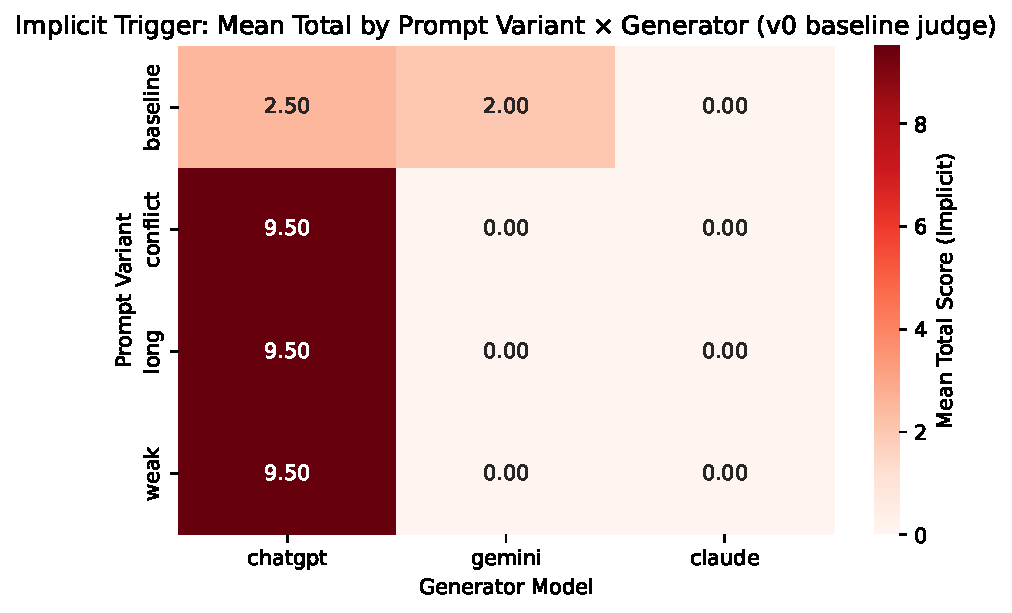
\includegraphics[width=0.92\linewidth]{figures/fig2_heatmap_v0.pdf}
  \caption{\textbf{Implicit-trigger mean total by prompt variant and generator family (v0).}
  Heatmap shows mean total scores under implicit triggers, highlighting strong heterogeneity across prompt variants and generator families.
  Numbers computed from the fixed snapshot under v0.
  Computed as $\mathrm{MT}(\pi)$ (Eq.~\ref{eq:mean-total}) with \texttt{trigger\_type=implicit}, grouped by \texttt{prompt\_variant} and \texttt{generator\_model}.}
  \label{fig:schema_cliff}
\end{figure}

\subsection{Instruction-following degradation beyond schema break}
\label{sec:quality}
Schema failures co-occur with broad quality degradation across rubric dimensions.
Under v0, the mean total score drops from 7.6875 (explicit) to 2.7500 (implicit) (max total = 10; fixed snapshot, v0).
Dimension means (each in $\{0,1,2\}$) also collapse. Let $(A,B,C,D,E)$ denote the rubric dimensions:
(A) structure; (B) snapshot constraint; (C) actionability; (D) completeness; (E) drift failure.
Dimension-level performance (on a 0--2 scale) reflects this collapse. Under explicit triggers, means across all five dimensions---including structure, actionability, and completeness---ranged from 1.25 to 1.67; under implicit triggers, these dropped to between 0.44 and 0.58.
Failure rates (fraction of examples with score $<2$) rise sharply across all dimensions.
For example, the failure rate for dimension \Edrift{} increases from $14/48$ (29.2\%) under explicit triggers to $40/48$ (83.3\%) under implicit triggers (fixed snapshot, v0).
Figure~\ref{fig:dim_pair} summarizes dimension-level breakdown and failure rates.

\begin{figure*}[t]
  \centering

  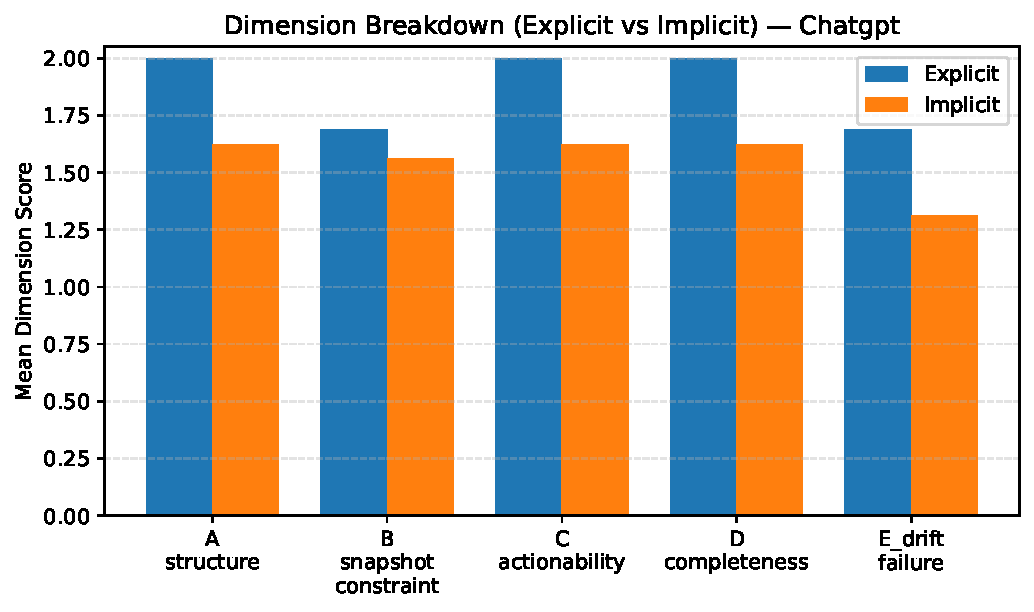
\includegraphics[width=0.47\linewidth]{figures/fig3_dimension_breakdown_chatgpt.pdf}\hfill
  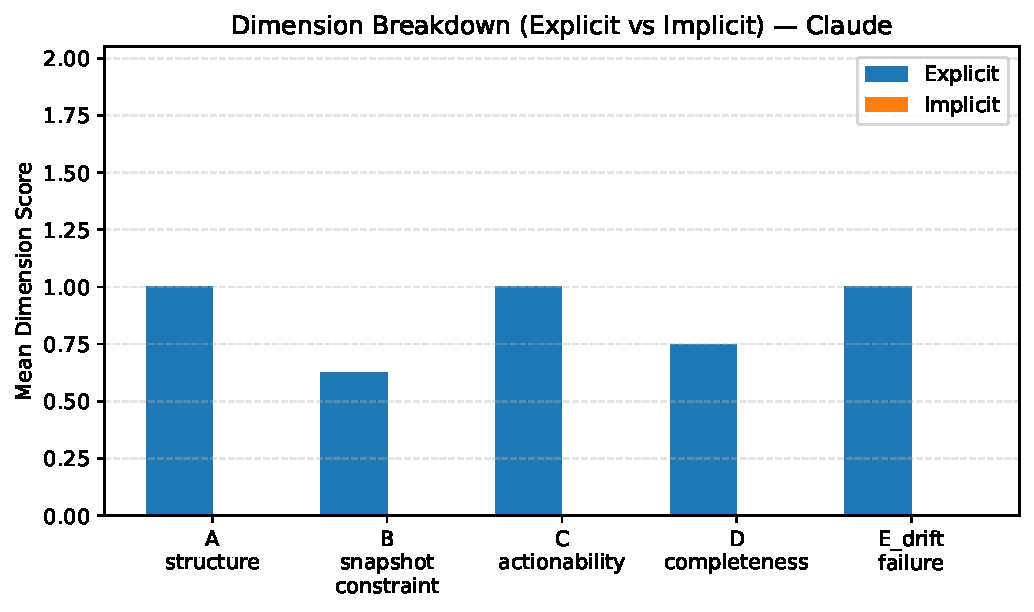
\includegraphics[width=0.47\linewidth]{figures/fig3_dimension_breakdown_claude.pdf}

  \vspace{4pt}

  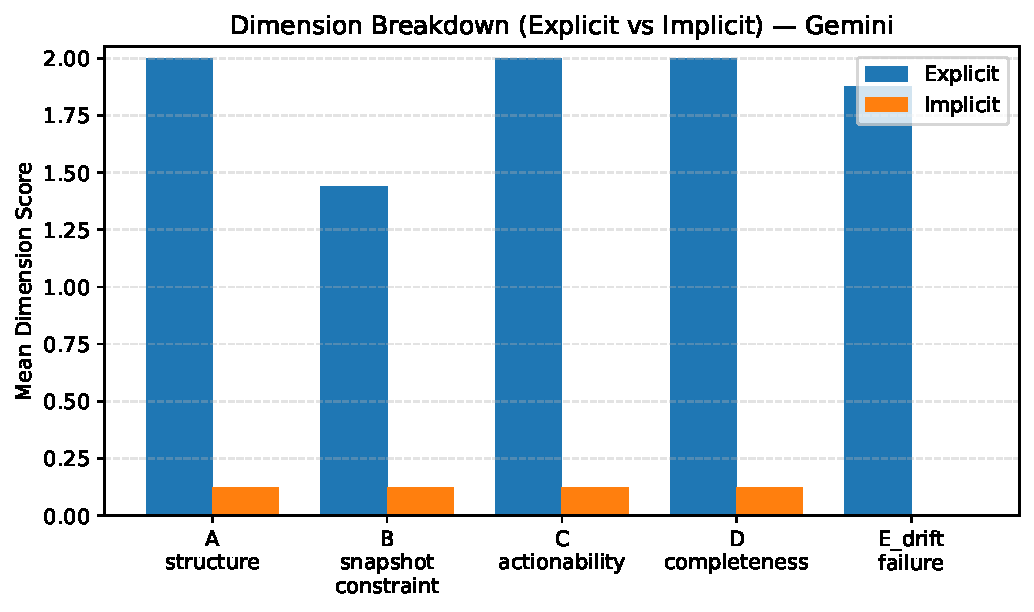
\includegraphics[width=0.47\linewidth]{figures/fig3_dimension_breakdown_gemini.pdf}\hfill
  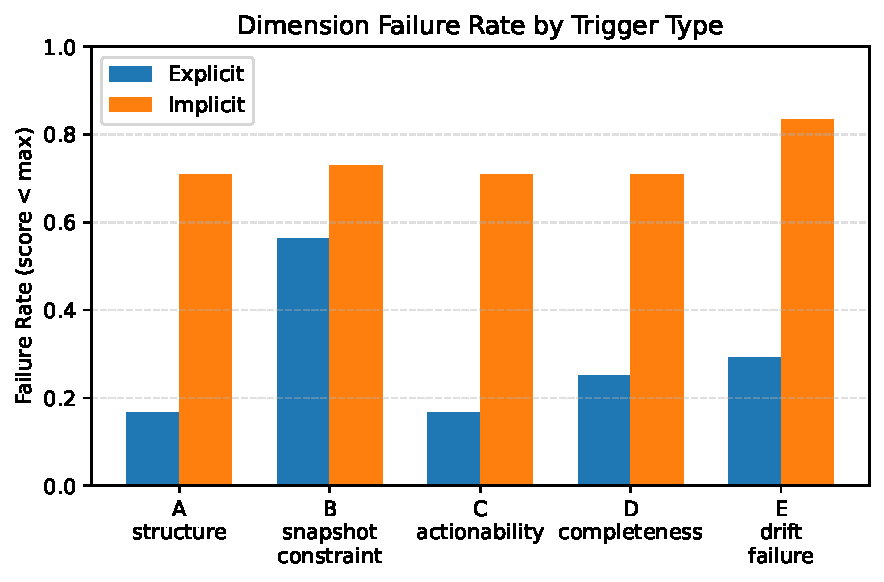
\includegraphics[width=0.47\linewidth]{figures/fig4_dimension_failure_rate.pdf}

  \caption{\textbf{Dimension-level degradation under implicit triggers (v0).}
  Mean scores by dimension for ChatGPT, Claude, and Gemini, plus failure rates (score $<2$) aggregated across generator families.
  Numbers are sourced from the fixed snapshot under v0.
  Top three panels are computed as $\mu_d(\pi)$ (Eq.~\ref{eq:dim-mean}); the failure-rate panel is computed as $\mathrm{DFR}_d(\pi)$ (Eq.~\ref{eq:dim-fail}) over frozen artifacts.}
  \label{fig:dim_pair}
\end{figure*}

\subsection{Slice-level diagnostics: why averages hide outages}
\label{sec:slices}
Operational monitoring must be slice-aware because failures concentrate.
We highlight three concrete slice patterns that are visible only when stratifying by question and prompt variant:

\paragraph{ChatGPT: Slice-Specific Resilience.}
Under implicit triggers, ChatGPT slices mostly retain high scores: among the eight slices (questions $q3$ and $q4$ across baseline, conflict, long and weak variants), only the $q4$--\emph{baseline} slice fully collapses with mean total $=0.0$ and a 100\% hard‑break rate ($2/2$).
The $q3$--\emph{baseline} slice shows partial degradation (mean total $=5.0$; hard‑break rate $1/2$), while the remaining six slices maintain high total scores ($\ge 9$) with zero hard‑breaks.
Thus, contract‑salience reduction is catastrophic only on specific slices rather than universally for ChatGPT.

\paragraph{Claude: Systemic Interface Failure.}
Claude outputs collapse across all slices under implicit triggers: for every combination of question ($q3,q4$) and prompt variant (baseline, conflict, long, weak), the mean total score is $0.0$ and the hard‑break rate is 100\% ($2/2$).
Implicit prompts therefore eliminate usable structure for Claude outputs.

\paragraph{Gemini: Context-Dependent Instability.}
Gemini outputs largely collapse under implicit triggers.
Across all eight slices, the mean total score drops to $0.0$ and the hard‑break rate is 100\% ($2/2$) except for the $q4$--\emph{baseline} slice, which retains partial structure (mean total $=4.0$; hard‑break rate $1/2$).
This heterogeneity again underscores that contract salience interacts strongly with both the generator and the task/variant context. Operationally, dashboards should report both global aggregates and worst-$k$ slices by hard-break rate and total-score drop.

\subsection{Judge-version sensitivity as a measurement incident}
\label{sec:judge}
Monitoring systems rely on LLM-based judges as instrumentation; judge prompt edits therefore
constitute instrumentation migrations that can shift reported severity on identical preserved outputs,
and should be interpreted as measurement risk rather than evidence of correctness.

\paragraph{Interpretation rule (instrument migration).}
We treat each judge prompt version as defining a distinct metric.
Therefore: (i) do not compare absolute scores across judge versions without an overlap-based calibration step, and (ii) do not pool or average metrics computed under different judge prompt versions.
Operationally, judge upgrades should be gated using overlapping preserved slices to bound expected metric shifts before changing dashboards or alerts.

\begin{sloppypar}
The fixed snapshot includes multiple judge versions applied to overlapping preserved outputs.
We highlight one overlapping slice with complete totals: ChatGPT-as-judge scoring Gemini-generated outputs under implicit triggers.
\end{sloppypar}
For this fixed set of 8 preserved outputs:
\begin{itemize}[leftmargin=1.2em, itemsep=2pt, topsep=2pt]
  \item v0 baseline judge: hard-breaks $8/8$; mean total = 0.0
  \item v1 paraphrased judge: hard-breaks $0/8$; mean total = 8.0 (range 7--9)
  \item v2 schema-strict judge: hard-breaks $0/8$; mean total = 10.0
\end{itemize}
All values are computed from preserved evaluation records for each judge version; no generator inference is re-run.
Figure~\ref{fig:judge_pair} further summarizes judge-version sensitivity.
In the fixed snapshot, v1/v2 are available for two overlapping judge/model slices---ChatGPT evaluating Gemini outputs and Gemini evaluating ChatGPT outputs---while the remaining slices are available only under v0.

  \begin{figure}[t]
  \centering
  
\includegraphics[width=0.92\linewidth]{figures/fig5_judge_comparison.pdf}
  \caption{\textbf{Judge-version sensitivity on preserved outputs.}  Comparison of v0, v1, and v2 under implicit triggers.  Numbers sourced from the fixed snapshot.
  Mean totals are computed as $\mathrm{MT}(\pi)$ (Eq.~\ref{eq:mean-total}); judge-version effects are summarized by $\Delta^{\text{judge}}_{m}$ (Eq.~\ref{eq:judge-delta}).
}
  \label{fig:judge_pair}
  \end{figure}

\section{Operational Implications}
We map the observed incident patterns to a CAO workflow.
\textbf{Catch} corresponds to interface validity and worst-slice monitors (detect outages early);
\textbf{Adapt} treats prompt edits as migrations with canaries and rollback;
\textbf{Operate} governs the judge as versioned instrumentation (pinning and no pooling across versions).

\subsection{Catch: monitor interface validity and slice-level metrics}
The first-line operational signal is \textbf{schema validity}.
Hard-break rates can be tracked continuously and alerted on as interface incidents.
Given strong heterogeneity (Section~\ref{sec:slices}), monitoring should also be \textbf{slice-aware}:
at minimum, stratify by generator family, question, and prompt variant.
A practical ``incident panel'' can be computed directly from row-level evaluation records without new experiments.

\subsection{Adapt: treat prompt edits as migrations, not refactors}
The schema cliff indicates that ``making prompts more natural'' by removing explicit markers can cause outages.
Two practical adaptation patterns follow:
(i) keep contract markers stable and implement stylistic polishing \emph{after} generation (rendering layer), and
(ii) deploy prompt edits via canaries with explicit rollback criteria based on schema and dimension-level monitors.
When a drift edit is required (policy updates), treat it as a migration with a pinned prompt version, rollback, and a post-mortem if hard-breaks exceed baseline.

\subsection{Operate: version and govern the judge as instrumentation}
Judge-version sensitivity is a measurement incident: instrument changes can flip conclusions.
We recommend three governance rules aligned with CAO:
\begin{itemize}[leftmargin=1.2em, itemsep=2pt, topsep=2pt]
  \item \textbf{Version pinning}: treat judge prompts as production dependencies with explicit version bumps.
  \item \textbf{No pooling across versions}: each judge version defines a distinct metric; compare only after overlap-based calibration.
 \item \textbf{Migration check}: gate upgrades using overlapping preserved slices to bound expected deltas.
\end{itemize}

\subsection{A minimal monitoring schema}
Table~\ref{tab:monitoring} lists a minimal monitoring schema computable from the fixed snapshot for CAO-style operations.
 
\begin{table}[t]
\centering
\small
\begin{tabular}{@{}p{0.24\linewidth}p{0.72\linewidth}@{}}
\toprule
\textbf{Signal} & \textbf{Definition (computed over the fixed snapshot)}\\
\midrule
Hard-break rate & $\mathrm{HBR}(\pi)$ (Eq.~\ref{eq:hbr}) by slice (question/variant/model)\\
Dim.\ failure rate & $\mathrm{DFR}_{d}(\pi)$ (Eq.~\ref{eq:dim-fail}) for each dimension $d$\\
Mean total & $\mathrm{MT}(\pi)$ (Eq.~\ref{eq:mean-total}) by slice and overall\\
Coverage & $n(\pi)$ (Eq.~\ref{eq:coverage}) preserved records in slice\\
Judge version & \texttt{judge\_version} (pinned evaluator prompt version)\\
\bottomrule
\end{tabular}
\caption{Minimal CAO monitoring schema computable from the fixed snapshot (no new experiments; deterministic aggregation only). All signals are computed from preserved evaluation records and their deterministic grouped summaries.}
\label{tab:monitoring}
\end{table}

\section{Limitations}
\paragraph{Scope boundary.}
Our evidence base is intentionally narrow and fixed: we analyze preserved artifacts rather than re-running generators/judges.
All quantitative claims are confined to the frozen evaluation slices (Q3--Q4).

\paragraph{Generalization and inference limits.}
We stop short of claiming statistical significance or i.i.d. generalization beyond these specific slices; counts such as $8/48$ denote matched evaluation records, not repeated samples.
We do not claim that any judge version is a ground-truth reference; observed cross-version shifts should be treated as calibration deltas requiring overlap checks.

\section{Conclusion}
Prompt-level drift is an operational monitoring problem.
Using a fixed-snapshot evidence base, we show that small prompt perturbations can trigger schema failure cliffs, degrade rubric-dimension scores, and shift evaluation conclusions when judge prompts change, with substantial slice-level heterogeneity.
These findings motivate CAO-style controls: monitor interface validity, treat prompt edits as migrations with rollback criteria, and govern judges as versioned instrumentation.

\section*{Reproducibility}
Code, prompts, processed evaluation snapshots, and figure-generation scripts are available at \url{https://github.com/yuchenzhu-research/iclr2026-cao-prompt-drift-lab}. 
All claims are based on frozen Q3--Q4 slices and the audit chain in Section~4 and Figure~1, and were verified against preserved outputs from the fixed snapshot.

\clearpage
\bibliographystyle{iclr2026_conference}
\bibliography{iclr2026_conference}

\end{document}